\begin{frame}{Introduction}
  \section{Introduction}
  \begin{columns}[T] 
    \begin{column}{0.5\textwidth}

    Ocean circulation gyres are part of the atmospheric circulation.
    \begin{enumerate}
    \item Heating air at the equator $\rightarrow$ Hadley cells.
    \item Coriolis effect deflects the air movement $\rightarrow$ Trade winds and westerlies
    \item Enforce wind stress on the ocean surface $\rightarrow$ 90\degr  Ekman transport.
    \item Since $f$ increases with latitude, net southward Ekman transport in the North Atlantic. 
    \item Western boundary current needed to close the circulation.
    \end{enumerate} 

    \end{column}
    \begin{column}{0.5\textwidth} 
      \begin{figure}
    \centering
    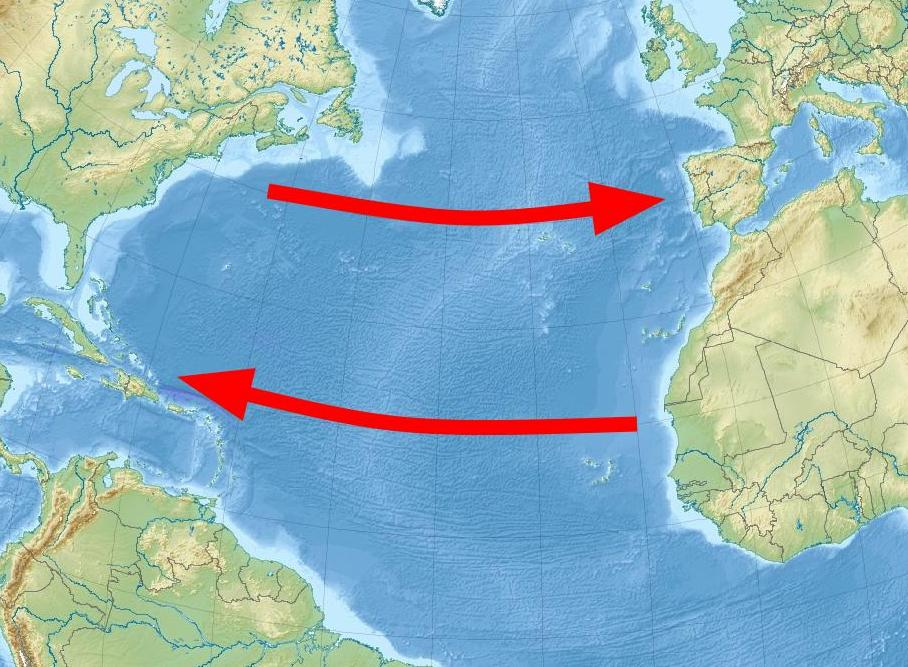
\includegraphics[width=\textwidth]{Figures/North_Atlantic.jpg}
    \caption{Wikimedia Commons, North Atlantic location map, accessed 2026}
  \end{figure}
    \end{column}
  \end{columns}
\end{frame}



\begin{frame}{Introduction, Sverdrup}
  \section{Theory}
  \subsection{Sverdrup}

  Harald Ulrik Sverdrup (1888-1957) formulated the net transport in the ocean interior as:

\begin{empheq}[box=\fbox]{equation}
  -\beta \frac{\partial \Psi}{\partial x} = \frac{1}{\rho}\nabla\times\vec{\tau}
\end{empheq}

which gives the Sverdrup solution:

\begin{equation*}
  \int_x^{x_\text{East}}\frac{\partial \Psi}{\partial x}\, dx = \int_x^{x_\text{East}} vH \, dx =
  \cancel{\Psi(x_\text{East},y)} - \Psi(x,y)
\end{equation*}
\begin{equation*}
  \implies\Psi(x,y) = -\frac{1}{\rho\beta}\int_x^{x_\text{East}} \left(\nabla\times\vec{\tau}\right) 
\end{equation*}
\end{frame}


\begin{frame}{Introduction, Munk}
  \subsection{Munk}

  Walter Heinrich Munk (1917-2019) extended the Sverdrup model by including meridional harmonic Newtonian viscosity (diffusion of momentum):
  \begin{empheq}[box=\fbox]{equation}
    A\nabla^4 \Psi -\beta \frac{\partial \Psi}{\partial x} = \frac{1}{\rho}\nabla\times\vec{\tau}
  \end{empheq}    

  which gives the Munk solution:
  \begin{align*}
    \Psi(x,y)=\Psi_{\text{Sverdrup}}(x,y)\Bigg(1-e^{-\frac{x-x_{\text{West}}}{2\delta_m}}\Bigg[ & \cos\!\left(\sqrt{3}\,\frac{x-x_{\text{West}}}{2\delta_m}\right)\\&+\frac{1}{\sqrt{3}}\sin\!\left(\sqrt{3}\,\frac{x-x_{\text{West}}}{2\delta_m}\right)\Bigg]\Bigg)
  \end{align*}

\begin{equation*}
  \text{ where } \delta_M\equiv\left(\frac{A}{\beta}\right)^{\tfrac{1}{3}}
\end{equation*}
\end{frame}


